\documentclass[11pt,a4paper]{article}
\newcommand{\docTitle}{EduTools Guide}
% preamble.tex --- shared LaTeX preamble for Choupo manuals
% Style: sober monochrome with subtle dark-blue accent for
% hyperlinks only.  Pedagogical boxes via tcolorbox.

% ---- Encoding, fonts, language --------------------------------------
\usepackage[utf8]{inputenc}
\usepackage[T1]{fontenc}
\usepackage{lmodern}
\usepackage[english]{babel}
\usepackage{microtype}
\usepackage{textcomp}

% ---- Layout ---------------------------------------------------------
\usepackage[a4paper, margin=2.4cm, headheight=15pt]{geometry}
\usepackage{fancyhdr}
\usepackage{titlesec}
\usepackage{enumitem}
\usepackage{longtable}
\usepackage{booktabs}
\usepackage{array}
\usepackage{tabularx}
\usepackage{multicol}
\usepackage{parskip}
\usepackage{needspace}
\usepackage{graphicx}

% ---- Code listings --------------------------------------------------
\usepackage{listings}
\usepackage{xcolor}

% Sober palette --- almost monochrome, one accent reserved for links
\definecolor{rulegray}{HTML}{888888}
\definecolor{lightgray}{HTML}{f4f4f4}
\definecolor{mediumgray}{HTML}{cccccc}
\definecolor{darkgray}{HTML}{555555}
\definecolor{accent}{HTML}{1c3a5a}

\lstdefinelanguage{dict}{
  morecomment=[l]{//},
  morecomment=[s]{/*}{*/},
  morestring=[b]",
}

\lstdefinelanguage{shell}{
  morecomment=[l]{\#},
}

\lstset{
  basicstyle=\ttfamily\footnotesize,
  backgroundcolor=\color{lightgray},
  frame=single,
  framerule=0.4pt,
  rulecolor=\color{mediumgray},
  numbers=none,
  showstringspaces=false,
  breaklines=true,
  breakatwhitespace=true,
  postbreak=\mbox{\textcolor{darkgray}{$\hookrightarrow$}\space},
  columns=fullflexible,
  keepspaces=true,
  xleftmargin=0.7em,
  framexleftmargin=0.7em,
  framextopmargin=0.5em,
  framexbottommargin=0.5em,
  commentstyle=\color{darkgray}\itshape,
  stringstyle=\color{black},
  language=shell,
  % No {---}/{--} -> en-dash rules: they mangle ASCII box art (the header
  % banner) and directory trees (|--...) and CLI --flags in listings.
  % Hyphens must stay literal in monospace.  Accents below ARE needed
  % (the listing font renders them via the LaTeX accent commands).
  literate={ã}{{\~a}}1 {á}{{\'a}}1 {â}{{\^a}}1
           {é}{{\'e}}1 {ê}{{\^e}}1
           {í}{{\'i}}1
           {ó}{{\'o}}1 {ô}{{\^o}}1 {õ}{{\~o}}1
           {ú}{{\'u}}1
           {ç}{{\c c}}1
           {·}{{\textperiodcentered}}1
}

% ---- PGFPlots (theory-guide figures) -------------------------------
\usepackage{pgfplots}
\pgfplotsset{compat=1.18}
\usetikzlibrary{arrows.meta, calc}

% ---- Boxes (pedagogical signposts) ----------------------------------
\usepackage[most]{tcolorbox}
\tcbuselibrary{breakable,skins}

\newtcolorbox{keyidea}{
  breakable,
  colback=lightgray,
  colframe=black,
  boxrule=0.4pt,
  arc=1pt,
  left=10pt,right=10pt,top=6pt,bottom=6pt,
  before upper={\noindent\textbf{\sffamily Key idea.}\quad},
}

\newtcolorbox{pitfall}{
  breakable,
  colback=white,
  colframe=darkgray,
  boxrule=0.4pt,
  arc=1pt,
  left=10pt,right=10pt,top=6pt,bottom=6pt,
  before upper={\noindent\textbf{\sffamily Common pitfall.}\quad},
}

\newtcolorbox{tryit}{
  breakable,
  colback=lightgray,
  colframe=darkgray,
  boxrule=0.4pt,
  arc=1pt,
  left=10pt,right=10pt,top=6pt,bottom=6pt,
  before upper={\noindent\textbf{\sffamily Try it now.}\quad},
}

\newtcolorbox{whatyoulllearn}{
  breakable,
  colback=white,
  colframe=black,
  boxrule=0pt,
  leftrule=2pt,
  arc=0pt,
  outer arc=0pt,
  left=10pt,right=4pt,top=2pt,bottom=2pt,
  before upper={\noindent\textit{\sffamily\small What you'll learn.}\quad},
}

% Worked example --- the pedagogical workhorse of the theory manual.
\newcounter{theoryexample}[section]
\renewcommand{\thetheoryexample}{\thesection.\arabic{theoryexample}}
\newtcolorbox{example}[1][]{
  breakable,
  colback=lightgray,
  colframe=black,
  boxrule=0.4pt,
  arc=1pt,
  left=10pt,right=10pt,top=6pt,bottom=6pt,
  title={\textbf{\sffamily Worked example~\thetheoryexample.}\enspace #1},
  fonttitle=\sffamily,
  coltitle=black,
  attach title to upper,
  before title={\refstepcounter{theoryexample}},
}

% Intuition --- a one-paragraph sense-making aside, marked by a left rule.
\newtcolorbox{intuition}{
  breakable,
  colback=white,
  colframe=black,
  boxrule=0pt,
  leftrule=2pt,
  arc=0pt,
  outer arc=0pt,
  left=10pt,right=4pt,top=2pt,bottom=2pt,
  before upper={\noindent\textit{\sffamily\small Intuition.}\quad},
}

% Link-back to a tutorial --- visual cue that this maps to a runnable case.
\newtcolorbox{tutoriallink}{
  breakable,
  colback=white,
  colframe=darkgray,
  boxrule=0pt,
  leftrule=2pt,
  arc=0pt,
  outer arc=0pt,
  left=10pt,right=4pt,top=2pt,bottom=2pt,
  before upper={\noindent\textbf{\sffamily\small Runnable case.}\quad},
}

% ---- Headers/footers ------------------------------------------------
\pagestyle{fancy}
\fancyhf{}
\renewcommand{\sectionmark}[1]{\markboth{\thesection\quad #1}{}}
\fancyhead[L]{\small\sffamily\nouppercase{\leftmark}}
\fancyhead[R]{\small\sffamily\thepage}
\fancyfoot[C]{\small\sffamily Choupo-2607}
\renewcommand{\headrulewidth}{0.3pt}
\renewcommand{\footrulewidth}{0pt}

\let\choupoSection\section
\renewcommand{\section}{\clearpage\choupoSection}

% ---- Section titles -------------------------------------------------
\titleformat{\section}
  {\Large\bfseries\sffamily}{\thesection}{0.8em}{}[\vspace{-0.4em}\rule{\linewidth}{0.3pt}]
\titleformat{\subsection}
  {\large\bfseries\sffamily}{\thesubsection}{0.8em}{}
\titleformat{\subsubsection}
  {\normalsize\bfseries\sffamily}{\thesubsubsection}{0.8em}{}

\titlespacing*{\section}{0pt}{2.0ex plus 1ex minus.2ex}{1.0ex plus.2ex}
\titlespacing*{\subsection}{0pt}{1.6ex plus 1ex minus.2ex}{0.8ex plus.2ex}

% ---- Hyperref last --------------------------------------------------
\usepackage[colorlinks=true,
            linkcolor=accent,
            citecolor=accent,
            urlcolor=accent,
            bookmarksnumbered=true,
            destlabel=true,        % \label{ch:cstr} -> PDF named destination "ch:cstr"
            pdfborder={0 0 0}]{hyperref}

% ---- Shortcuts ------------------------------------------------------
\newcommand{\code}[1]{\texttt{#1}}
\newcommand{\file}[1]{\texttt{#1}}
\newcommand{\dict}[1]{\texttt{#1}}
\newcommand{\cpp}{C\texttt{++}}

% Manual authorship is selected by each guide before loading this preamble.
% Properties/Theory: Vitor, Pedro, Miguel. All other guides: Vitor alone.
\newcommand{\manualauthors}{%
  \ifdefined\propertyTheoryAuthors
    V\'{\i}tor Geraldes, Pedro Mendes, and Miguel Rodrigues%
  \else
    V\'{\i}tor Geraldes%
  \fi}

% OpenFOAM-style manual front matter: title page, then a copyright/licence
% notice page.  No source-code banner belongs on manual covers.
\newcommand{\manualfrontmatter}[2]{%
  \begin{titlepage}
  \thispagestyle{empty}
  \vspace*{2.0cm}
  \begin{center}
  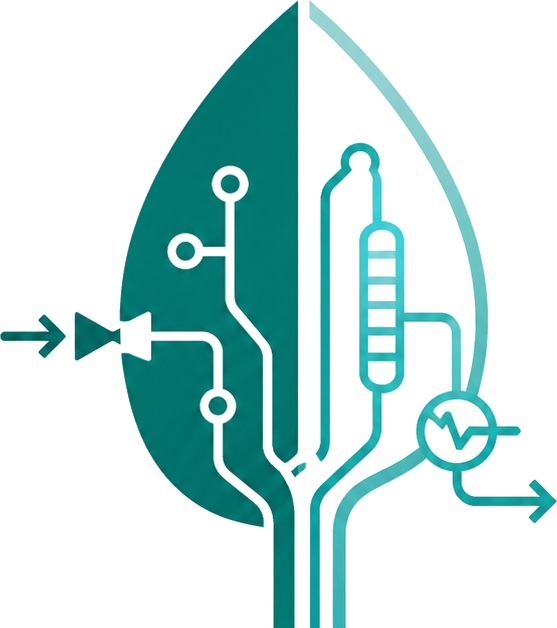
\includegraphics[height=4.0cm]{../gui/public/logo2-mark.png}\\[0.8cm]
  {\Huge\bfseries\sffamily Choupo}\\[0.35cm]
  {\Large\sffamily The Open Source Chemical Process Simulator}\\[1.3cm]
  {\Huge\bfseries\sffamily #1}\\[0.7cm]
  {Version 2607}\\[0.1cm]
  {30 June 2026}
  \end{center}
  \end{titlepage}

  \clearpage
  \thispagestyle{empty}
  \vspace*{1.2cm}
  \noindent Copyright \textcopyright{} 2026 \manualauthors.\\[0.3cm]
  \noindent Authors: \manualauthors.\\[0.3cm]
  \noindent This work is licensed under a Creative Commons
  Attribution-ShareAlike 4.0 International License.\\[0.3cm]
  \noindent Code examples, Choupo case files, and other machine-readable
  examples are licensed under GPL-3.0-or-later.\\[0.3cm]
  \noindent Typeset in \LaTeX.

  \vspace{1.0cm}
  \noindent\rule{\linewidth}{0.3pt}
  \noindent\footnotesize\textit{Acknowledgment.}\quad Choupo was conceived and
  architected by V\'{\i}tor Geraldes. Substantial parts of the initial
  implementation, documentation, and tutorial corpus were produced with
  assistance from Anthropic Claude Code using Claude Opus/Fable models. This
  guide is published under human curation, review, and editorial responsibility
  by \manualauthors.

  \clearpage
  \markboth{License}{License}
  \section*{License}
  \lstinputlisting[
    basicstyle=\ttfamily\tiny,
    frame=none,
    backgroundcolor=\color{white},
    breaklines=true,
    columns=fullflexible
  ]{cc-by-sa-4.0.txt}

  \clearpage
  \markboth{Trademarks}{Trademarks}
  \section*{Trademarks}
  #2
  \clearpage
}


\title{}
\author{}
\date{}

% ---------------------------------------------------------------------
%  Local shortcuts.  No new packages: everything below is built from what
%  preamble.tex already loads.
% ---------------------------------------------------------------------

% A pointer INTO the Theory Guide.  This guide never restates a derivation:
% it names the destination and stops.  The argument is the PDF named
% destination (hyperref destlabel=true makes every \label in the Theory
% Guide one), so the string printed here is the same string the tool's
% registry entry carries and the same string the book icon opens.
% \theorydest and \declaredanchor moved to preamble.tex (2026-08-30): the
% Theory Guide's ch:solubility-parameter now uses \declaredanchor too, and a
% per-guide copy of a shared macro is the arity sin -- the guide that lacked
% it simply failed to compile, silently served stale.
\newcommand{\derivation}[1]{%
  \smallskip\noindent\textbf{\sffamily\small Derivation.}\quad #1\par\smallskip}

\begin{document}

\manualfrontmatter{EduTools Guide}{
Choupo is a trademark of TalentGround Lda.

Anthropic, Claude, and Claude Code are trademarks or registered trademarks of
Anthropic, PBC.

OpenFOAM is a registered trademark of OpenCFD Ltd.
}

% =====================================================================
%   Table of contents
% =====================================================================
\pagenumbering{roman}
\setcounter{tocdepth}{1}
\markboth{Contents}{Contents}
\tableofcontents
\clearpage
\pagenumbering{arabic}
\setcounter{page}{1}

% =====================================================================
\section{What this guide is --- and what it is not}\label{sec:edu-what}

EduTools is the plane of Choupo's browser application where the
\emph{classical graphical methods} are constructed over curves the engine
computes: the McCabe--Thiele staircase, the Kremser recovery curve, the
$\varepsilon$--NTU chart, the Levenspiel plot, the Van~Heerden
ignition diagram, the pinch composite curves, and the rest.  Each tool
draws a construction a student has met on paper, on numbers a real solver
produced, and puts the method's answer beside the engine's.

\begin{keyidea}
This guide is a \textbf{lesson companion}, not a theory manual.  It says
what each construction is \emph{for}, what to turn, what to watch, and
what the picture is silent about.  It contains no derivations at all.
\end{keyidea}

That absence is deliberate and it is architectural.  Every equation behind
these tools already has exactly one home --- \file{docs/theoryGuide.pdf} ---
and every live tool declares, in its registry entry, the named destination
in that guide where its derivation lives.  A second document carrying the
same derivations would be a second home for the same statement, and within
one semester the two would disagree.  So this guide \emph{points}, and the
Theory Guide \emph{derives}.  When you want to know why
$\varepsilon = (1-e)/(1-C_r e)$, follow the pointer.  When you want to know
what a class will get wrong about it, you are in the right document.

\subsection*{The five questions each tool section answers}

Every tool documented here is written to the same five headings, in the
same order, because a lesson is more portable than a description:

\begin{enumerate}[leftmargin=*,nosep,topsep=2pt]
  \item \textbf{The question} --- in one sentence a student would recognise
        from a problem sheet.
  \item \textbf{What to vary, what to watch} --- the specific knob that
        makes the lesson visible, and what should happen when you turn it.
  \item \textbf{The misconception the construction exposes} --- what
        students actually get wrong, not merely what is true.  This is the
        part worth reading twice.
  \item \textbf{What the picture does not say} --- the limits of the
        construction.  In this project that is treated as part of teaching
        it, never as an apology for it.
  \item \textbf{Where the derivation lives} --- a pointer into the Theory
        Guide, never a copy of it.
\end{enumerate}

\subsection*{Where the other material is}

\begin{itemize}[leftmargin=*,nosep]
  \item \textbf{Theory Guide} --- every derivation, every hypothesis, every
        worked example.  The authority for all physics.
  \item \textbf{Explorer Guide} --- the \emph{property surfaces}
        ($T$-$x$-$y$, $\gamma(x)$, $P^{\mathrm{sat}}$ scans).  The split
        criterion between the two planes is stated in the application
        itself: method-construction $\rightarrow$ EduTools,
        property-surface $\rightarrow$ Explorer.
  \item \textbf{Tutorials Guide} --- the runnable cases.  Every EduTools
        tool runs one of them; this guide names which.
  \item \textbf{User Guide} --- authoring cases on disk, which is where any
        finding from a tool should end up.
\end{itemize}

% =====================================================================
\section{How a tool feeds itself}\label{sec:edu-feeding}

\begin{whatyoulllearn}
Where the numbers on the screen come from, why a tool works with no case
open, and what a knob is actually allowed to change.
\end{whatyoulllearn}

\subsection{Opening a tool}

EduTools is a tab of its own.  The tool chooser leads the chrome row on
that tab; on a case tab showing EduTools in its body the chooser is one
slim row above the construction.  Either way the list is the same, and a
construction that is on the roadmap but not yet built is shown
\emph{disabled} rather than hidden --- the menu states the roadmap instead
of implying it.

Every tool is deep-linkable:

\begin{lstlisting}[language=shell]
?workspace=methods&tool=<id>
\end{lstlisting}

\noindent
The \code{methods} key is a contract and does not change with the
workspace's caption, so a link already in a student's notes goes on
working.  The tool identifiers are the ones listed in
\S\ref{sec:edu-tools} and \S\ref{sec:edu-stubs}.

Under the chooser sits a one-line caption of what the construction
teaches, and beside it a book icon that opens the Theory Guide \emph{at
this tool's own section}.  That icon is the pointer this whole guide is
built around: a tool that cannot name its derivation is not finished, and
a test in the application refuses an anchor the Theory Guide does not
define.

\subsection{Classroom, or your own run}

Most tools default to \textbf{Classroom}: the tool clones a bundled
tutorial --- its \emph{witness} case --- writes your knob values into that
case's own dictionary files, and solves it in the browser with the
WebAssembly build of the same solver the command line runs.  Nothing needs
to be open, and nothing on disk is touched.

When the application's current run also carries the surfaces a tool reads,
a source toggle offers \textbf{Current run} beside the classroom witness.
A tool that a run cannot feed says so and stays empty; it never draws
something else wearing the same name.

\begin{keyidea}
A knob turns a \emph{declared scalar} in the witness's dictionary and
nothing else.  The engine then recomputes everything.  A knob that cannot
find its key fails loudly rather than silently doing nothing, and a knob
that would not reach the physics is deliberately absent --- each absence
recorded with its reason in the tool's own source.
\end{keyidea}

That last rule has teeth.  Several plausible-looking controls are missing
on purpose: a pressure that a liquid-phase rate law never reads would be a
placebo control; an integrator step count sitting beside physical knobs
invites reading numerics as physics; a kinetic pre-exponential that a
witness deliberately re-tuned would leave the tool teaching a case other
than the one it names.

\subsection{Why the picture can be trusted}

Three standing rules govern this plane, and they are worth telling a class
about, because they are the reason the construction and the simulator
cannot quietly diverge.

\begin{enumerate}[leftmargin=*,nosep,topsep=2pt]
  \item \textbf{No physics in the browser.}  Every curve is an engine
        column, an engine KPI, or an engine-written report file.  The
        browser draws.
  \item \textbf{Method geometry is the one exception, and it is
        labelled.}  A staircase, a trapezoid area, a textbook closed form,
        a heat cascade re-run over published curves --- these \emph{are}
        the method being taught, so a few tools own them.  Where that
        happens the tool says so on screen, and the engine's own number is
        the judge: agreement is verification, and a disagreement is a
        finding about the drawing, never a moved answer.
  \item \textbf{An absence stays an absence.}  A number the engine did not
        publish is not rendered as zero and not invented.  Solver
        advisories are lifted out of the run log and shown, because these
        tools have no log tab to bury them in.
\end{enumerate}

\begin{pitfall}
A tool that shows nothing is usually telling you something.  ``This run
publishes no Van~Heerden surface'' means the reactor you solved was
isothermal --- there is no generation-versus-removal diagram for it.  The
honest empty state is a diagnosis; read it before changing the tool.
\end{pitfall}

% =====================================================================
\section{The constructions}\label{sec:edu-tools}

Six constructions are documented in full below.  The remaining six live
tools are listed in \S\ref{sec:edu-stubs} with what is missing from each,
because a thin lesson is worse than an admitted gap.

The six were chosen to span the three transfer subjects a course actually
has to cover, two constructions each, and to prefer the tools whose
\emph{misconception} is both common and hard to dislodge by telling:

\begin{itemize}[leftmargin=*,nosep]
  \item \textbf{Mass transfer} --- McCabe--Thiele
        (\S\ref{sec:edu-mccabe}) and Kremser (\S\ref{sec:edu-kremser}).
  \item \textbf{Heat transfer} --- $\varepsilon$--NTU
        (\S\ref{sec:edu-entu}) and pinch composite curves
        (\S\ref{sec:edu-pinch}).
  \item \textbf{Reaction} --- Levenspiel (\S\ref{sec:edu-levenspiel}) and
        Van~Heerden (\S\ref{sec:edu-vanheerden}).
\end{itemize}

% ---------------------------------------------------------------------
\subsection{Distillation: the McCabe--Thiele staircase}\label{sec:edu-mccabe}

\declaredanchor{ch:distillation}

\subsubsection*{The question}

\emph{A binary feed of composition $x_F$ is to be split into a distillate
$x_D$ and a bottoms $x_W$.  At reflux ratio $R$ and feed quality $q$, how
many equilibrium stages does it take, and on which stage does the feed
enter?}

\subsubsection*{What to vary, what to watch}

\begin{tryit}
Set a sharp split ($x_D = 0.95$, $x_W = 0.05$, $x_F = 0.5$), then drag
$R$ \emph{down} toward the red $R_{\min}$ tick on the slider.  Watch three
things at once: the staircase steps multiply, the \emph{approach to pinch}
bar fills and reddens, and at $R \le R_{\min}$ the construction stops
with a banner naming the pinch abscissa.  Then drag $R$ up and watch how
little the stage count changes once you are clear of the cliff.
\end{tryit}

\begin{itemize}[leftmargin=*,nosep]
  \item \textbf{$R$} --- the primary knob.  The slider can be bound to
        $R$ directly or to $R/R_{\min}$; the second binding is the design
        lens (``$1.3\times$ minimum'') and makes the cliff a fixed
        landmark at $1.0$ instead of a number that moves.
  \item \textbf{$q$} --- rotates the $q$-line about $(x_F, x_F)$.  Watch
        the feed-stage index move, and watch $R_{\min}$ itself change:
        the same column, the same specifications, a different minimum
        reflux, because the feed arrived hotter or colder.
  \item \textbf{$E_{MV}$} --- the Murphree tray efficiency.  Below $1$ the
        staircase steps to a dashed \emph{pseudo}-curve and the count
        becomes a count of real trays.
  \item \textbf{The partial-condenser switch} --- adds exactly one
        equilibrium stage, and the readout says so.
  \item \textbf{The components, $\gamma$ model and $P$} --- these are the
        only settings that re-run the engine, because they are the only
        ones that change the equilibrium curve.  Everything else redraws
        instantly.
\end{itemize}

\subsubsection*{The misconception the construction exposes}

\begin{pitfall}
\textbf{That the equilibrium curve responds to the reflux ratio.}  It is
the commonest confusion in the whole subject, and it is usually invisible
because on paper the student redraws the entire figure each time.  Here the
curve is a frozen engine result and the staircase is pure geometry over it,
so turning $R$ at sixty frames a second while $y^{*}(x)$ does not so much
as flicker makes the point physically: \emph{reflux is an operating
decision; the equilibrium curve is a statement about the mixture}.  Change
the pressure or the activity model and the engine re-runs and the curve
moves --- which is the same lesson from the other side.
\end{pitfall}

Two further confusions the same picture settles:

\begin{itemize}[leftmargin=*,nosep,topsep=4pt]
  \item \textbf{That $R_{\min}$ is a property of the column.}  It is the
        intersection of the $q$-line with the equilibrium curve --- feed
        composition, feed quality, product specifications and
        thermodynamics, and no equipment at all.  Turn $q$ and $R_{\min}$
        moves although nothing has been built or unbuilt.
  \item \textbf{That more reflux is better because it needs fewer
        stages.}  The chart shows only one half of that trade.  Stage
        count falls steeply just above $R_{\min}$ and then flattens; the
        vapour traffic $V = (R+1)D$, and with it the reboiler duty, the
        condenser duty and the column diameter, goes on rising linearly
        and is \emph{nowhere on this diagram}.  A student who optimises on
        the staircase alone will choose a column that cannot be paid for.
\end{itemize}

\subsubsection*{What the picture does not say}

\begin{itemize}[leftmargin=*,nosep]
  \item \textbf{The operating lines are straight because Constant Molar
        Overflow is assumed.}  The tool states this permanently under the
        chart rather than in a footnote.  CMO is an energy assumption
        (equimolar latent heats), and it is the one thing on the diagram
        that is not the real model.  The equilibrium curve, by contrast,
        is the real curve at that pressure --- not a constant-$\alpha$ toy.
  \item \textbf{No energy, no hydraulics, no diameter.}  There is no
        reboiler duty, no condenser duty, no pressure drop, no flooding
        check.  A column that is impossible to build converges perfectly
        well here.
  \item \textbf{Stages are not trays} unless $E_{MV} < 1$, and $E_{MV}$
        is a \emph{declared} number --- from a correlation, a chart, or
        plant data.  The engine will not invent it.
  \item \textbf{The azeotrope you see belongs to the declared model.}  If
        no curated binary-interaction pair covers the system, the tool
        announces that it is drawing \emph{ideal} mixing and that the
        diagram therefore cannot show an azeotrope at all.  Read that
        banner: an absent azeotrope may be a fact about the mixture or a
        fact about the data coverage, and only the banner tells you which.
  \item \textbf{Binary only.}  A third component has no axis here.
\end{itemize}

\subsubsection*{Where the derivation lives}

\derivation{Theory Guide, \emph{Distillation column, Wang-Henke
bubble-point} (\theorydest{ch:distillation}) --- the stage model, CMO, and
the rigorous column this construction is the hand method for.  The closed
forms for the two limits the staircase locates geometrically,
$N_{\min}$ and $R_{\min}$, are derived in \emph{Shortcut distillation:
Fenske--Underwood--Gilliland} (\theorydest{ch:fug}).  The Murphree
efficiency and its effective-$K$ treatment are in \emph{Tray hydraulics}
(\theorydest{ch:hydraulics}).  The staircase construction itself ---
horizontal to the operating line, vertical to the equilibrium curve --- is
drawn and explained in the absorber chapter
(\theorydest{ch:absorber}), where the same geometry serves a
counter-current cascade.}

% ---------------------------------------------------------------------
\subsection{Absorption: the Kremser shortcut, judged}\label{sec:edu-kremser}

\declaredanchor{ch:absorber}

\subsubsection*{The question}

\emph{A gas carrying a soluble solute is washed counter-currently with a
lean solvent.  How much of the solute do $N$ stages recover --- and does
the one-line shortcut agree with what the column actually does?}

\subsubsection*{What to vary, what to watch}

The construction has two halves and the lesson is in the gap between them.
The curve is the Kremser closed form, recovery against $N$ at the
absorption factor $A = L/(KV)$ the engine published.  The point is the
engine's own stagewise recovery for the column that was solved.  The chip
between them is the labelled deviation.

\begin{tryit}
Start from the witness (an ammonia/water absorber, six stages, both feeds
at $298.15$~K).  Now raise the ammonia in the gas feed, step by step, and
watch \emph{two} chips together: \code{dT\_rise} climbing as more heat of
absorption is released, and the deviation between the shortcut and the
column growing with it.  Then put the ammonia back and raise the solvent
flow instead: $A$ rises, recovery rises, and the deviation shrinks.
\end{tryit}

\begin{itemize}[leftmargin=*,nosep]
  \item \textbf{Stages $N$} --- the knob students reach for first.  Watch
        how quickly the curve flattens: past a handful of stages, more
        stages buy very little.
  \item \textbf{Solvent flow $L$} --- the knob that actually moves the
        answer, because it moves $A$.
  \item \textbf{Solute feed flow} --- the knob that breaks the shortcut,
        by making the column non-isothermal.
  \item \textbf{Feed temperatures} --- both of them, gas and solvent, with
        the \code{nonIsothermal} flag and \code{dT\_rise} as the readout.
\end{itemize}

\subsubsection*{The misconception the construction exposes}

\begin{pitfall}
\textbf{That the deviation is an error.}  A student who has only met the
closed form reads any gap between shortcut and simulator as a defect ---
a bad $K$, a loose tolerance, a bug.  It is neither.  Kremser assumes
\emph{one constant} $A$, which means a straight operating line and a
straight equilibrium line, which means an isothermal column.  Absorption
is exothermic.  The solvent heats as it descends, $K$ rises with
temperature, and $A = L/(KV)$ therefore \emph{falls} exactly where the
column is doing its work.  The engine re-evaluates $K$ stage by stage; the
shortcut cannot.  The gap is the assumption failing, and it is real.
\end{pitfall}

The direction matters as much as the size, and it is the part worth
labouring: for a soluble, exothermic solute the isothermal Kremser is
\emph{optimistic}.  It promises recovery the column will not deliver.  A
shortcut that erred the other way would merely be conservative; this one
sends you to site with a column that underperforms.

A second confusion, milder but persistent:

\begin{itemize}[leftmargin=*,nosep,topsep=4pt]
  \item \textbf{That $A > 1$ settles the matter.}  $A$ is a ratio of two
        slopes, not a pass mark.  At $A$ barely above one, recovery
        approaches its ceiling so slowly that no realistic stage count
        gets there; at $A$ comfortably above one, a few stages do almost
        everything.  The curve makes the difference between those two
        situations obvious in a way that the inequality $A > 1$ never can.
\end{itemize}

\subsubsection*{What the picture does not say}

\begin{itemize}[leftmargin=*,nosep]
  \item \textbf{The $A$ on the chip is a single number for a column whose
        $K$ varies.}  It is evaluated at the feed temperature.  That is
        precisely why the two sides of the deviation chip are not the same
        calculation --- and precisely what makes the chip informative.
  \item \textbf{Absorbers only.}  A stripper publishes a stripping factor
        $S = KV/L$ and a temperature \emph{drop}, not these keys, so it
        does not activate this tool.  That is a correct refusal, not a
        missing feature: the mirrored construction is a different lesson.
  \item \textbf{Stages are theoretical.}  No packing height, no HETP, no
        tray efficiency, no flooding.
  \item \textbf{No solvent circuit.}  The lean solvent arrives lean.  A
        real plant regenerates it, and the regenerator's residual solute
        sets a floor on the recovery that no stage count can beat.  That
        loop is not on this diagram.
\end{itemize}

\subsubsection*{Where the derivation lives}

\derivation{Theory Guide, \emph{Absorber and stripper: the counter-current
cascade} (\theorydest{ch:absorber}).  The absorption factor
$A_i = L/(K_i V)$ and the tridiagonal stage system are in \emph{The
counter-current cascade and the absorption factor}; the reason the engine
does not use the closed form, and the temperature bulge that makes the
isothermal shortcut optimistic, are in \emph{Why the energy balance
matters}.}

% ---------------------------------------------------------------------
\subsection{Heat exchange: effectiveness against NTU}\label{sec:edu-entu}

\declaredanchor{ch:hx-entu}

\subsubsection*{The question}

\emph{I have an exchanger of area $A$ and overall coefficient $U$, and two
streams with known inlet temperatures and flows.  What duty do I actually
get --- and if I want more, will more area give it to me?}

\subsubsection*{What to vary, what to watch}

The chart is the family of $\varepsilon(\mathrm{NTU})$ curves at several
capacity ratios $C_r$, with the solved exchanger's own point placed on the
curve for its own $C_r$.  A chip reports whether the drawn geometry
reproduces the engine's effectiveness; when it does not, that is a
statement about the configuration the tool assumed, never about the point.

\begin{tryit}
Double the area, from $10$ to $20$~m\textsuperscript{2}, and read the duty
before and after.  Then double it again, to $40$.  Note how much of the
first doubling you got back on the second.  Now set the two heat-capacity
rates far apart (raise one flow, drop the other), so $C_r \to 0$, and
switch between counter-current and co-current: the two curves close up
until they lie on top of each other.
\end{tryit}

\begin{itemize}[leftmargin=*,nosep]
  \item \textbf{Area $A$ and coefficient $U$} --- both enter only through
        $\mathrm{NTU} = UA/C_{\min}$, which is the first thing to notice:
        a better coefficient and a bigger exchanger are the same move on
        this chart.
  \item \textbf{The two flows} --- they set $C_{\min}$, $C_{\max}$ and
        hence both $\mathrm{NTU}$ and $C_r$, so a flow change slides the
        point along one curve \emph{and} moves it to another.
  \item \textbf{The two inlet temperatures} --- they do not move the point
        at all.  They set $Q_{\max}$, and therefore the duty in kilowatts,
        but $\varepsilon$, $\mathrm{NTU}$ and $C_r$ are all independent of
        them.  Verifying that is a good five minutes.
  \item \textbf{The configuration} --- counter-current, co-current, or one
        shell with two tube passes.
\end{itemize}

\subsubsection*{The misconception the construction exposes}

\begin{pitfall}
\textbf{That duty scales with area.}  $\mathrm{NTU}$ is linear in $A$;
$\varepsilon$ is emphatically not.  Every curve on the chart bends over,
and past roughly $\mathrm{NTU} = 3$ the return on further area is nearly
nothing --- the exchanger is already delivering most of what the inlet
temperatures permit, and no amount of metal buys what thermodynamics has
capped.  Students who have only seen $Q = UA\,\Delta T_{LM}$ read a
proportionality that is not there, because $\Delta T_{LM}$ collapses as
the exchanger gets good.
\end{pitfall}

The second one is more interesting, and the chart proves it in one move:

\begin{itemize}[leftmargin=*,nosep,topsep=4pt]
  \item \textbf{That counter-current is always better.}  It is never
        worse, but at $C_r = 0$ --- one stream condensing or boiling, or
        simply so large that its temperature barely moves --- the two
        arrangements give \emph{identical} effectiveness, and the curves
        coincide exactly.  The advantage of counter-current flow is
        purchased entirely by the temperature change of the smaller
        stream, so when that change is absent there is nothing to buy.
        This is worth doing on the screen because it is the kind of fact
        that is remembered as a slogan and applied where it does not hold.
  \item \textbf{That $\varepsilon$ is an efficiency, so $\varepsilon =
        0.75$ means a quarter is wasted.}  Nothing is wasted;
        the exchanger is adiabatic to its surroundings and every joule
        that leaves the hot stream arrives in the cold one.  $\varepsilon$
        is normalised by $Q_{\max} = C_{\min}(T_{h,\mathrm{in}} -
        T_{c,\mathrm{in}})$, a ceiling set by the \emph{inlet
        temperatures}, which is a statement about what an infinitely
        large exchanger could do --- not about losses.
\end{itemize}

\subsubsection*{What the picture does not say}

\begin{itemize}[leftmargin=*,nosep]
  \item \textbf{It is a rating result, not a design.}  ``Given this
        hardware, what happens?'' is the question answered.  ``What
        hardware do I need?'' is a different loop, with pressure drop and
        geometry in it.
  \item \textbf{No pressure drop, no fouling, no cost.}  The chart's flat
        tail says extra area stops paying in duty; it says nothing about
        what the area costs, and nothing about the pumping power the extra
        length consumes.
  \item \textbf{Heat-capacity rates are taken as constant} across the
        pass.  A stream whose $c_p$ swings, or which changes phase part
        way, is outside the assumption.
  \item \textbf{Three configurations only.}  Cross-flow arrangements, and
        the correction factors that go with them, are not offered here.
\end{itemize}

\subsubsection*{Where the derivation lives}

\derivation{Theory Guide, \emph{Two-stream heat exchanger: the
$\varepsilon$--NTU rating method} (\theorydest{ch:hx-entu}) --- the
definitions of $C_r$ and $\mathrm{NTU}$, the counter-current and
co-current closed forms, the duty from $Q_{\max}$, and the
$UA\,\mathrm{LMTD} = Q$ self-check.  The design problem the rating chart
does not answer --- geometry, pressure drop, the sizing loop --- is the
section immediately following it, \emph{Heat exchanger DESIGN}.}

% ---------------------------------------------------------------------
\subsection{Heat integration: the composite curves and the pinch}\label{sec:edu-pinch}

\declaredanchor{ch:pinch}

\subsubsection*{The question}

\emph{Before a single exchanger is drawn: what is the least hot utility
and the least cold utility this set of streams can possibly need?}

\subsubsection*{What to vary, what to watch}

The tool draws the engine's own published composite curves, reports its
targets $Q_{H,\min}$ and $Q_{C,\min}$ and the pinch temperature, re-runs
the heat cascade over the published curves as a cross-check, and renders
the engine's candidate-match table verbatim.

\begin{tryit}
Change nothing but $\Delta T_{\min}$ --- from $20$~K down to $10$, then up
to $30$.  Watch the composite curves slide together and apart, the two
targets move in opposite directions, and the pinch temperature itself
change.  Nothing physical has been altered: not a stream, not a flow, not
a temperature.  Ask the class what, then, has changed.
\end{tryit}

\begin{itemize}[leftmargin=*,nosep]
  \item \textbf{$\Delta T_{\min}$} --- the decisive knob, and the one that
        is a \emph{choice}.
  \item \textbf{The supply temperatures} --- move one stream's start and
        watch whether the pinch stays where it was.  Sometimes it does
        not, and the region boundaries in the candidate table move with it.
  \item \textbf{The flows} --- a flow scales that stream's $CP$, which
        changes the slope of its segment of the composite curve.  A steep
        segment and a flat one are the same duty over different
        temperature spans.
  \item \textbf{The candidate table} --- read the temperature-feasibility
        column and the pinch-rule column separately.  A match may be
        thermodynamically possible and still violate the $CP$ rule at the
        pinch.
\end{itemize}

\subsubsection*{The misconception the construction exposes}

\begin{pitfall}
\textbf{That the pinch is a property of the plant.}  It is a property of
the stream data \emph{plus a number the engineer chose}.  Turning
$\Delta T_{\min}$ moves the pinch temperature and both targets while the
process stands still.  Students routinely quote ``the pinch is at
$115^{\circ}$C'' as though it had been measured; it was assumed into
existence, half of it by the choice of driving force, and the value of
that choice is an economic trade-off between exchanger area and utility
bill that this pass does not make for you.
\end{pitfall}

Two more, and the third is the one that decides coursework marks:

\begin{itemize}[leftmargin=*,nosep,topsep=4pt]
  \item \textbf{That a target is a design.}  The table lists
        \emph{thermodynamically admissible candidates} and never ranks
        them.  The word ``optimal'' does not appear anywhere in this pass,
        and a gate in the test suite enforces that.  Reaching the target
        may require more exchangers, and more awkwardly placed ones, than
        anybody would build; plot plan, control, start-up and safety are
        not in the temperature table.
  \item \textbf{That heating below the pinch merely costs a little
        extra.}  It costs \emph{exactly its own duty}, and so does cooling
        above the pinch, and the two are additive:
        \[
          \sum(\text{heating below}) + \sum(\text{cooling above})
          \;=\; Q_{H,\mathrm{current}} - Q_{H,\min}.
        \]
        The violation diagnostics report both sums, and they are computed
        by different code from the targets --- so the identity closing is
        a check you can do by hand and the tool can fail.  A student who
        has only the slogan ``do not transfer heat across the pinch''
        cannot say how much a violation costs; this identity says exactly
        how much.
\end{itemize}

\subsubsection*{What the picture does not say}

\begin{itemize}[leftmargin=*,nosep]
  \item \textbf{Energy targets only.}  Area targets, capital targets, and
        the capital-versus-energy trade-off that would let you
        \emph{choose} $\Delta T_{\min}$ economically are a further phase
        and are not implemented.  The Theory Guide states this in the same
        words rather than describing something the engine does not have.
  \item \textbf{It never rewrites the network.}  The flowsheet you wrote
        is the flowsheet that ran; the pass analyses it and stops.
  \item \textbf{A unit enters as its net duty.}  A column with a reboiler
        and a condenser is a single net number unless you model the two as
        separate units --- and for a column that is usually the wrong
        picture.  Splitting is the fix, and it is your decision, not the
        pass's.
  \item \textbf{The grand composite curve is derived in view.}  The engine
        publishes the hot, cold and shifted composite curves; the tool
        builds the grand composite from those, and labels it as such.  The
        cross-check chip exists so you can see that the derivation
        reproduces the engine's targets.
\end{itemize}

\subsubsection*{Where the derivation lives}

\derivation{Theory Guide, \emph{Pinch analysis: the target before the
network} (\theorydest{ch:pinch}) --- the $CP$ line, why $\Delta T_{\min}$
shifts the axes, the problem table cascade by cascade, the composite
curves, the candidate matches, the violation identity, and an explicit
\emph{What this pass does not do}.}

% ---------------------------------------------------------------------
\subsection{Reactor sizing: the Levenspiel plot}\label{sec:edu-levenspiel}

\declaredanchor{ch:pfr}

\subsubsection*{The question}

\emph{The same reaction, the same feed, the same conversion --- which
reactor is smaller, a plug-flow tube or a stirred tank, and by how much?}

\subsubsection*{What to vary, what to watch}

One chart carries $1/(-r_A)$ against conversion $X_A$, and on it two
areas: the plug-flow reactor's integral $\int_0^{X_{\mathrm{out}}}
\mathrm{d}X/(-r_A)$ under the curve, and the stirred tank's rectangle of
height $1/(-r_A)$ \emph{at the outlet} and width $X_{\mathrm{out}}$.  Both
witnesses are twins --- byte-identical feed, kinetics and thermodynamics
--- so the comparison is between reactors and never between chemistries.

\begin{tryit}
Raise the plug-flow reactor's volume so $X_{\mathrm{out}}$ climbs, and
watch the rectangle and the area separate.  At low conversion they nearly
coincide; at high conversion the rectangle towers over the area.  Then
lower the temperature: the whole curve lifts (a slower rate is a larger
ordinate) and both reactors grow --- but the \emph{ratio} between them is
governed by the curve's shape, not its height.
\end{tryit}

\begin{itemize}[leftmargin=*,nosep]
  \item \textbf{Reactor temperature} --- through the Arrhenius constant.
  \item \textbf{The two feed flows} --- the limiting reactant sets
        $F_{A0}$ and the co-reactant changes what the rate law sees.
  \item \textbf{The plug-flow volume} --- the knob that walks
        $X_{\mathrm{out}}$ along the curve, which is the axis the whole
        lesson lives on.
\end{itemize}

\subsubsection*{The misconception the construction exposes}

\begin{pitfall}
\textbf{That the stirred tank needs more volume because it is somehow a
worse reactor.}  Students reach for a hardware explanation --- poorer
mixing, dead zones, short-circuiting.  The chart shows that the cause is
the opposite and is purely geometric: a stirred tank is \emph{perfectly}
mixed, so every molecule in it sits at the outlet composition and
therefore at the outlet rate --- the \emph{lowest} rate anywhere in the
duty.  The tube sees the whole range of rates from inlet to outlet.  The
rectangle circumscribes the area because perfect mixing throws away every
fast rate the reaction was willing to give.  \emph{Being well mixed is
what costs the volume.}
\end{pitfall}

And immediately after that, the guard against over-learning it:

\begin{itemize}[leftmargin=*,nosep,topsep=4pt]
  \item \textbf{That ``a CSTR always needs more volume'' is a law.}  It
        follows from the curve \emph{rising} with conversion, which is
        what positive-order kinetics do.  Draw a rate law whose
        $1/(-r_A)$ has a minimum --- autocatalysis, strong product
        inhibition --- and the rectangle can be the smaller of the two
        over part of the range, which is why real plants sometimes put a
        tank first and a tube after it.  The construction is valuable
        exactly because it is a picture and not a rule: it shows you how
        to check, on any kinetics, rather than what to remember.
  \item \textbf{That the smaller reactor is the cheaper one.}  Volume is
        not price.  A large stirred tank can be considerably cheaper than
        a small tubular reactor with the same duty once you count
        fabrication, catalyst containment, cleaning and control.
\end{itemize}

\subsubsection*{What the picture does not say}

\begin{itemize}[leftmargin=*,nosep]
  \item \textbf{The comparison is isothermal.}  Both witnesses run at the
        same declared temperature.  Nothing here shows the thermal
        behaviour that makes the two reactors genuinely different animals
        --- for that, go to \S\ref{sec:edu-vanheerden}.
  \item \textbf{No residence-time distribution.}  Plug flow and perfect
        mixing are the two ideal limits; every real reactor is between
        them, and neither line on this chart is a real vessel.
  \item \textbf{Reversible kinetics are clipped, and the clipping is
        announced.}  Past equilibrium the engine's rate goes negative and
        those points are excluded from the area, with the exclusion stated
        in the chart annotation.  An integral run through them would be
        arithmetic, not physics.
  \item \textbf{The stirred tank's volume is not a knob here}, for a
        recorded reason: the witness declares it inline, out of reach of
        the override grammar the classroom knobs use.  It always runs its
        authored value.  This is stated in the tool's own provenance line
        rather than left to be discovered.
\end{itemize}

\subsubsection*{Where the derivation lives}

\derivation{Theory Guide, \emph{Plug-flow reactor} (\theorydest{ch:pfr})
--- the differential balance, the RK4 integration, and the first-order
analytic check that gives the canonical comparison at $k\tau = 1$
($X^{\mathrm{PFR}} = 1 - e^{-1} = 0.632$ against $X^{\mathrm{CSTR}} =
1/(1+k\tau) = 0.500$), which is this construction in closed form for one
special case.  The stirred tank's own extent formulation is in
\emph{Continuous stirred-tank reactor} (\theorydest{ch:cstr}).}

% ---------------------------------------------------------------------
\subsection{Multiple steady states: the Van~Heerden diagram}\label{sec:edu-vanheerden}

\declaredanchor{ch:cstr}

\subsubsection*{The question}

\emph{The same reactor, the same feed, the same everything --- so why does
it sometimes sit cold and sometimes run hot, and could it be made to sit
in between?}

\subsubsection*{What to vary, what to watch}

The diagram is heat \textbf{generated} $G(T)$ against heat
\textbf{removed} $R(T)$, both drawn from the engine's own scan of the
reactor's steady-state equation.  Generation is a sigmoid: the rate rises
exponentially with temperature and then saturates once the reactant is
gone.  Removal is a straight line, because in an adiabatic vessel the only
sink is the sensible heat that leaves with the product.  A straight line
can cut a sigmoid three times.

\begin{tryit}
Drag \code{T\_guess} slowly from $280$~K to $430$~K and watch the
\emph{reported} marker.  For a long stretch nothing happens; then it jumps
to another crossing on a diagram that has not moved at all.  Same
equipment, same feed, same equations --- a different answer, decided by
where you started.  That is not a numerical artefact; it is why real
reactors have a start-up procedure.
\end{tryit}

\begin{itemize}[leftmargin=*,nosep]
  \item \textbf{\code{T\_guess}} --- the decisive knob.  The engine finds
        \emph{all} the roots, prints them, and reports the one nearest
        your guess.
  \item \textbf{Feed temperature} --- slides the removal line.  Push it up
        far enough and the two lower crossings merge and vanish; the
        reactor can then only be ignited.
  \item \textbf{Reactor volume} --- stretches the generation sigmoid
        against a removal line that does not move with it.
  \item \textbf{The \code{steadyStates} count and the ignition span} ---
        how many crossings there are, and how far the reactor jumps
        between the coldest and the hottest.
\end{itemize}

\subsubsection*{The misconception the construction exposes}

\begin{pitfall}
\textbf{That three answers means the solver is broken.}  Students trained
on ``the equation has \emph{an} answer'' read multiplicity as a defect ---
a bad initial guess, a tolerance too loose, a bug to be reported.  It is
the physics of the system, and the diagram is the proof: an exponential
generation curve and a linear removal line intersect three times over a
range of conditions, and each intersection is a genuine steady state of
the same hardware.  The initial guess is not a numerical convenience in
this problem.  It is the start-up procedure, written as a number.
\end{pitfall}

The one that is harder, and better:

\begin{itemize}[leftmargin=*,nosep,topsep=4pt]
  \item \textbf{That the middle state is merely difficult to converge
        to.}  It is not difficult; it is \emph{unstable}.  A steady-state
        solver will sit on it happily, which is exactly what makes it
        dangerous pedagogy: the number exists and the reactor cannot hold
        it.  Nudge the temperature up and generation exceeds removal, so
        it climbs further; nudge it down and it falls to the extinguished
        state.  ``The solver converged'' and ``the plant can run there''
        are different claims, and this is the cleanest demonstration in
        the corpus that the second does not follow from the first.
  \item \textbf{That the ignited state is the one you want.}  It is the
        one with the conversion.  It may also be past a selectivity
        limit, past a catalyst's sintering temperature, or past the
        vessel's design pressure --- none of which appear on a diagram
        whose only axes are temperature and heat.
\end{itemize}

\subsubsection*{What the picture does not say}

\begin{itemize}[leftmargin=*,nosep]
  \item \textbf{It is a steady-state diagram.}  It says which states
        \emph{exist}.  It does not say how the reactor travels between
        them, how long ignition takes, whether it overshoots, or what the
        transient does to the catalyst.  That is the dynamic simulator's
        subject.
  \item \textbf{The instability flag is an ordering, not an analysis.}
        With exactly three roots the tool marks the middle one, which is
        arithmetic on the engine's own root list.  With any other count it
        makes \emph{no} stability claim at all --- a restraint worth
        pointing out to a class, because it is the difference between a
        result and a habit.
  \item \textbf{The removal line is straight because this reactor is
        adiabatic.}  Add a cooling jacket at a fixed coolant temperature
        and it is still straight, with a different slope and intercept;
        let the coolant temperature vary along the vessel and it is not
        straight at all, and the geometry of ``how many crossings'' has to
        be re-argued.
  \item \textbf{The kinetics are a declared teaching variant.}  The
        witness's own header says so, and its Arrhenius parameters are
        deliberately \emph{not} knobs: a construction about start-up
        should not silently become a construction about a different
        chemistry.
\end{itemize}

\subsubsection*{Where the derivation lives}

\derivation{Theory Guide, \emph{Continuous stirred-tank reactor}
(\theorydest{ch:cstr}) --- the material balance in the reaction extent and
the one-dimensional solve the engine performs, which is the equation whose
roots this diagram displays.  The witness case
\file{tutorials/steady/reactors/cstr05\_multiplicity} carries the
generation-versus-removal argument in its own \file{flowsheetDict} header,
and is the fullest written statement of the construction in the tree; the
tool quotes it.}

% =====================================================================
\section{The correlation library, and how to read a disagreement}
\label{sec:edu-correlations}

Every construction in \S\ref{sec:edu-tools} rests on correlations, and a
simulator normally hides them.  It picks one, computes with it, and prints
a number.  The student learns that the friction factor \emph{is} $0.0223$,
in the same tone of voice the simulator uses for the molar mass of water.

It is not.  It is one correlation's answer, and which one was chosen is
part of the answer.

This section is about the instruments that make that visible.  They are
not charts --- they run under \code{choupoProps} and print --- but they
teach something no chart can, because the thing to be seen is a
\emph{disagreement between authorities}, and a chart of one curve cannot
show it.

\subsection{What a correlation carries}

A correlation in Choupo is an object, and it is required to answer four
questions about itself:

\begin{itemize}[leftmargin=*,nosep,topsep=2pt]
  \item \textbf{What am I?} --- the expression, evaluated.
  \item \textbf{Where do I stop being valid?} --- the window its own
        authors stated, in words, printed on every run.
  \item \textbf{Who says so?} --- a dated primary citation.  A correlation
        whose source lives in a code comment is one the reader cannot
        check.
  \item \textbf{Can I still prove it?} --- a \emph{verify} against a
        published anchor, re-run every time, with the deviation printed
        beside the source.
\end{itemize}

The fourth is the unusual one.  A self-check that nobody wires up is a
promise, not a check; running it on every use is what turns it into one.

\subsection{The friction factor: four answers to one question}
\label{sec:edu-friction}

\declaredanchor{ch:hydraulics-pressure}

\subsubsection*{The question}

\emph{Water at $\mathrm{Re} = 10^{5}$ in a commercial steel line,
$\varepsilon/D = 10^{-3}$.  What is the Darcy friction factor?}

Run \code{tutorials/props/hydraulics/moody01\_friction\_correlations} and
four correlations answer:

\begin{center}
\begin{tabular}{lll}
\toprule
correlation & $f$ & \\
\midrule
Blasius     & $0.017770$ & \textbf{outside its window} \\
Churchill   & $0.022343$ & \\
Colebrook   & $0.022175$ & \\
Haaland     & $0.021966$ & \\
\midrule
\multicolumn{2}{l}{spread over all four} & $25.74\,\%$ \\
\multicolumn{2}{l}{spread over the three inside their windows} & $1.72\,\%$ \\
\bottomrule
\end{tabular}
\end{center}

\subsubsection*{The two numbers, and why there are two}

Read the last two rows together, because either one alone is misleading.

\emph{The correlations disagree by 26\,\%} is what the first row says, and
it is false.  Three of them agree within $1.7\,\%$ --- which for a
correlated quantity is agreement, not disagreement.

What produces the $25.74\,\%$ is Blasius, and Blasius is not wrong.  It is
being \emph{misused}.  Blasius carries no roughness term at all: it was
fitted to smooth pipes and knows nothing about a wall.  Asked about
$\varepsilon/D = 10^{-3}$ it answers anyway, confidently, twenty per cent
low, and there is nothing about the number $0.017770$ that looks wrong.

That is the whole content of a validity window, and it is why this run
prints one for every correlation on every call.  The window is not
bureaucracy attached to the formula.  It is the only thing standing
between a plausible number and a reader.

\begin{tryit}
Set \code{relRough} to $0$ --- a hydraulically smooth pipe --- and run
again.  Blasius comes back inside its window, the two spreads collapse
onto each other, and the four answers agree to a few per cent.  Now raise
\code{relRough} to $10^{-2}$ and watch the gap between the two spreads
widen: the more the wall matters, the more expensive Blasius's silence
about it becomes.

Then set \code{Re} to $1500$.  Three of the four announce that they have
substituted the exact laminar law $f = 64/\mathrm{Re}$, because they are
turbulent fits and say so.  Churchill does not need to: its single
expression contains the laminar law as its own limit, which is why it is
the default and why its self-check is anchored there.
\end{tryit}

\subsubsection*{What the anchors actually test --- and it differs}

The run prints a deviation for each correlation against a published
anchor.  It would be easy to read four small numbers as four validations.
They are not the same kind of statement, and the output says which is
which:

\begin{itemize}[leftmargin=*,nosep,topsep=2pt]
  \item \textbf{Blasius} is checked against its own closed form.  This
        tests the \emph{arithmetic} and nothing else --- and the run says
        so, so that a deviation of $0.000\,\%$ cannot be mistaken for
        agreement with a measurement.
  \item \textbf{Colebrook} is checked in the fully-rough limit, where its
        implicit equation collapses to a closed form.  This tests that the
        fixed-point iteration \emph{arrives}.
  \item \textbf{Haaland} is checked against \emph{Colebrook}, because
        agreement within about $2\,\%$ is precisely the claim Haaland
        published.  Anchoring him to anything else would be checking a
        claim nobody made.
  \item \textbf{Churchill} is checked against the exact laminar law.  This
        is the strongest of the four: it is a property the expression was
        built to have and that no coding error preserves by accident.
\end{itemize}

\subsubsection*{What the picture does not say}

\textbf{None of these four is checked against experimental data.}  Choupo
carries no friction measurements at all.  Two of the anchors are
self-consistency by construction and one is agreement with another
correlation; only Colebrook's tests an algorithm against a closed form the
equation itself provides.  The run passes, and what it establishes is that
the code computes what the papers wrote --- not that the papers are right.

The bench also never says which correlation to use.  That depends on the
pipe: its roughness, whether the flow is developed, whether the duct is
even circular.  A tool that ranked them would be making the engineer's
decision quietly, which is exactly what a silent default does.

And nothing here speaks about the transition band,
$2300 < \mathrm{Re} < 4000$, where no correlation was regressed and the
flow itself is not single-valued.  Correlations evaluated there are marked
outside their window, and that mark is the entire answer available.

\subsection{One family so far}

This discipline covers the convective heat-transfer correlations
(\code{heatTransferBench}) and, since 2026-08-25, the friction factor
(\code{frictionBench}).  It does \emph{not} yet cover the rest: the engine
computes Wilke--Chang, Chilton--Colburn, Thiele, Weisz, Joback,
Lee--Kesler, Rackett and Watson, and those remain internal to the
operations that use them --- correct, cited in comments, and invisible to a
student.

Saying so is the point.  A guide that implied an exhaustive catalogue
where two families exist would be committing the error this whole section
is about: presenting one answer as though it were the only one.

% =====================================================================
% =====================================================================
\section{One number for ``like dissolves like''}
\label{sec:edu-solubility}

A student asked to pick a solvent has a shelf of bottles and no way to
rank them.  The oldest useful answer is a single number per liquid, and
it is worth teaching precisely because it is \emph{almost} right --- the
places where it fails are as instructive as the places where it works.

\subsection{Where the number comes from}

Vaporising a liquid pulls its molecules apart.  The energy that costs,
per unit volume, is the \emph{cohesive energy density}; its square root
is Hildebrand's solubility parameter:

\begin{equation}
  \delta \;=\; \sqrt{\frac{\Delta H_{\mathrm{vap}}(T) - RT}{V_m}}
  \label{eq:hildebrand}
\end{equation}

Two things in that expression are worth stopping on.

The $RT$ is the work the vapour does pushing the atmosphere aside.
Subtracting it turns an \emph{enthalpy} of vaporisation into an
\emph{energy} of vaporisation, and only the second one measures cohesion.
Leaving it in gives a $\delta$ a few per cent high --- small enough to
look right, which is what makes it a favourite error.

And $\delta$ is a function of temperature that nobody writes the
temperature next to.  As a liquid approaches its critical point the
cohesive energy goes to zero, and so does $\delta$: there is no longer a
liquid to pull apart.  Published tables are at $25\,^\circ$C; a
$\delta$ quoted without a temperature is a number from an unstated state.

\subsection{Running it}

\begin{center}
\code{choupoProps} with a \code{solubilityParameter} operation.
\end{center}

Choupo \emph{derives} $\delta$ --- it is never stored.  Every input is
already in the component record (the latent heat at $T_b$, the critical
temperature, the liquid molar volume), so a stored $\delta$ would be a
second home for a fact the record already fixes, free to drift from it.
The latent heat at $T$ comes from the same Watson correlation the
enthalpy legs use, not a second copy of it.

The output has three parts: what each substance's $\delta$ is and what it
was computed from; how far that sits from an independently published
value where the record carries one; and the pairwise table
$|\delta_i - \delta_j|$, which is what the question actually was.

\subsection{The column that makes it checkable}

\begin{tryit}
Look at the \emph{published} column before you look at anything else.

Equation~\ref{eq:hildebrand} has three chances to go quietly wrong: a unit
slip in $V_m$, the missing $RT$, and reporting $\mathrm{Pa}^{0.5}$ where
the literature uses $\mathrm{MPa}^{0.5}$ --- a factor of $31.6$ that still
looks like a solubility parameter.  None of the three raises an error.

What catches them is that some records carry a $\delta$ somebody else
computed, independently, and the run prints the deviation.  Across the
substances where both exist the derivation reproduces the published value
to well under a per cent; a deviation of several per cent is therefore a
\emph{finding} and not noise.

This is the same device as the $Z_c$ column in a property data bank: a
redundant determination turns a plausible wrong number into a visible
disagreement.  A tool that computes something you cannot check is a tool
that is right until the day it is not.
\end{tryit}

\subsection{Where one number stops}

\textbf{Hildebrand carries no hydrogen bonding.}  Ethanol
($\delta \approx 26~\mathrm{MPa}^{1/2}$) and nitromethane
($\approx 25.1$) sit almost on top of each other, and a formulator
knows they behave differently --- one donates hydrogen bonds and the
other does not.  The theory cannot express the difference, because it
compressed every kind of intermolecular force into one scalar.

That is why the coatings industry uses Hansen's three-way split:
dispersion, polar and hydrogen-bonding contributions, with miscibility
judged by a distance in that space rather than on a line.  Choupo does
\emph{not} implement it, and the run says so every time: Hansen's
parameters are a separate dataset this project does not hold.

So the honest reading of a close pair is \emph{candidate}, never
\emph{verdict} --- and the run prints exactly that sentence, on every
call, rather than letting a small number imply more than it carries.

\begin{tryit}
Put water in the list.  Its $\delta$ is enormous
($\approx 48~\mathrm{MPa}^{1/2}$), far from every organic on
the shelf, and the pairwise table will duly report that water mixes with
nothing.  Water and ethanol are of course miscible in all proportions.

That single row is the clearest lesson the tool gives: the number is a
measure of \emph{how much} energy holds a liquid together, and says
nothing about \emph{what kind}.
\end{tryit}

\section{Constructions not yet documented here}\label{sec:edu-stubs}

Six live tools are \emph{not} written up above.  They are listed here with
what exists and what is missing, because an admitted gap is a better guide
than six thin sections.  Each is a working tool: what is absent is the
lesson material, not the construction.

For every entry below, what is missing is the same three things:

\begin{itemize}[leftmargin=*,nosep,topsep=2pt]
  \item the \textbf{misconception} the construction exposes --- the part
        that has to be observed in a classroom before it can be written
        down, and the part that cannot be guessed from the source;
  \item \textbf{what the picture does not say} --- the limits, stated
        with the same care as the six above;
  \item a \textbf{worked ``what to vary, what to watch''} sequence, tried
        on the tool rather than inferred from its knobs.
\end{itemize}

\subsection*{Psychrometric chart \quad(\code{tool=psychro})}
The humid-gas state map: saturation, relative-humidity lines,
adiabatic-saturation and true wet-bulb lines, over any carrier gas and
condensable pair the catalogue can serve.  Every line is engine-computed.
\declaredanchor{ch:drying}

\subsection*{Drying curve, batch tray \quad(\code{tool=drying})}
The two classical drying plots side by side on one run --- moisture
against time, and rate against moisture --- with the critical moisture
visible as the corner where a flat rate begins to fall.  The tool is
careful about one thing that deserves writing up properly: the engine
omits the break time entirely when the crossing was never observed, and
the tool reports \emph{which} absence it is rather than drawing a zero.
\declaredanchor{ch:drying}

\subsection*{Cooling tower, Merkel \quad(\code{tool=merkel})}
The saturated-air enthalpy curve above, the operating line below, and the
gap between them shaded --- that gap is the driving force the packing has
to buy.  A chip holds the four-point Chebyshev hand method against the
engine's converged integral.
\declaredanchor{ch:coolingTower}

\subsection*{Batch still, Rayleigh \quad(\code{tool=rayleigh})}
The graphical Rayleigh integration: the area under $1/(y^{*} - x)$ between
the pot's final composition and the charge \emph{is} $\ln(W_0/W)$, drawn
over the engine's own equilibrium curve and judged against the engine's
rigorously integrated still.
\declaredanchor{ch:rayleigh}

\subsection*{Pump against system curve \quad(\code{tool=pump-system})}
The operating point as an intersection: the pump's pressure rise falling
with flow against the pipe system's demand rising with it.  The tool is
explicit that the ``pump curve'' is whatever the pump \emph{model}
published, and greys it out with the caveat spelled in full when the model
was specified by a fixed pressure rise and the curve is therefore the
specification echoed back.
\declaredanchor{ch:rotating}

\subsection*{Adsorption breakthrough \quad(\code{tool=breakthrough})}
The S-shaped breakthrough curve against the ideal square wave drawn at the
engine's stoichiometric time: the mass-transfer zone consumes bed capacity
long before the bed is saturated.
\declaredanchor{ch:adsorption}

% =====================================================================
\section{Using a tool in a lesson}\label{sec:edu-lesson}

Three patterns that work, drawn from how the tools are built rather than
from how they could be used.

\subsection*{Turn one knob, and predict first}

Every classroom tool re-solves in the browser on each knob change, which
makes the interesting move cheap: ask for a prediction, then turn the
knob.  The productive knobs are the ones whose consequence is
counter-intuitive --- $\Delta T_{\min}$ on the pinch tool, area on the
$\varepsilon$--NTU chart, \code{T\_guess} on the Van~Heerden diagram, the
solute loading on the Kremser tool.  All four are documented above with
what should happen.

\subsection*{Make the deviation chip the discussion}

Several tools put a classical hand method beside the engine's answer and
report the gap.  That gap is the lesson, and its size is not the point ---
its \emph{cause} is.  On the Kremser tool the gap is the isothermal
assumption failing, and it grows the more exothermic the duty.  On the
cooling-tower tool the gap is nearly zero, and saying so plainly rather
than manufacturing drama is itself worth modelling for students: a hand
method that reproduces a converged integral to five figures has been
\emph{validated}, and that is a result.

\subsection*{Read the refusal}

An engine that refuses is teaching.  A pinched McCabe--Thiele
construction, an infeasible cooling tower, an absorber whose stripper twin
does not activate the tool, a drying run that never reached its critical
moisture --- each of those is a message with a reason in it.  The tools
show the engine's own words verbatim rather than a generic failure, and
the reason is usually the physics of the case rather than a mistake in the
input.

\begin{keyidea}
All models are wrong; some are useful.  Everything in this plane is built
so a student can see \emph{which} assumption is doing the work --- and
what happens on the day it stops being true.
\end{keyidea}

% =====================================================================
\section{Notes for maintainers}\label{sec:edu-maintenance}

\subsection*{One anchor, and it must resolve}

Each tool's registry entry names a Theory Guide destination.  The preamble
shared by all the manuals sets \code{destlabel=true}, so every
\code{\textbackslash label} in the Theory Guide becomes a PDF named
destination and the book icon jumps straight to it.  An anchor the guide
does not define fails \emph{silently} in a browser --- the PDF simply
opens at page one --- so a test in the application checks every declared
anchor against the guide source.  A tool without a resolvable anchor is
not finished.

\subsection*{Anchors are chapter-level, and some chapters are broader than
their tool}

The declared anchor points at the section that owns the tool's \emph{unit
operation}, which is not always the section that derives the tool's
\emph{construction}.  Where the two differ, the \emph{Where the derivation
lives} paragraphs above name both destinations rather than pretending the
first covers everything.  Two cases are worth knowing about before adding
a seventh tool section:

\begin{itemize}[leftmargin=*,nosep]
  \item A construction may be the hand method for a chapter that derives
        the \emph{rigorous} model instead --- the staircase against the
        stagewise column, the Levenspiel areas against the differential
        balance.
  \item A construction may be argued most fully in its \emph{witness
        case's} own dictionary header rather than in the manual.  That is
        a real source and this guide cites it as one, but it is not a
        substitute for a derivation, and a section that has to reach for
        it is flagging a gap in the Theory Guide rather than filling one.
\end{itemize}

\subsection*{When a tool changes}

A knob added or removed, a chip relabelled, a witness re-parameterised:
each of those can invalidate a \emph{What to vary, what to watch} block
here, and none of them will fail a build.  The blocks are written to name
knobs by their on-screen labels so a mismatch is at least visible to a
reader with the tool open.  Prose staleness is deliberately not gated in
this project --- a text search cannot tell a live claim from a recorded
one --- so the check is human, and it belongs in the same change that
touches the tool.

\end{document}
